\documentclass{beamer}
\usepackage[utf8]{inputenc}
\usepackage{graphicx, epsfig}
\usepackage{amsmath,mathrsfs,amsfonts,amssymb}
\usepackage{subfig}
\usepackage{floatflt}
\usepackage{epic,ecltree}
\usepackage{mathtext}
\usepackage{fancybox}
\usepackage{fancyhdr}
\usepackage{bm}
\usepackage{multirow}
\usepackage{enumerate}
\usepackage{epstopdf}
\usepackage{multicol}
\usetheme{Copenhagen}%{Singapore}%{Warsaw}%{Warsaw}%{Darmstadt}
\usecolortheme{whale}
%\definecolor{beamer@blendedblue}{RGB}{15,120,80}

\newcommand{\T}{{\text{\tiny\sffamily\upshape\mdseries T}}}
%--------------------------------------------------------------------------------
\title[\hbox to 56mm{Human Activity Recognition  \hfill\insertframenumber\,/\,\inserttotalframenumber}]
{Generative models for human activity recognition}
\author[ROY team]{\\
	{\small \textbf{ROY team:} Ilya Zharikov, \\ \hspace{2.67cm}Roman Isachenko, \\ \hspace{2.61cm}Artem Bochkarev}}
\institute[SkolTech]{Skolkovo Institute of Science and Technology \\
	Machine Learning course 
	\vspace{0.3cm}
}
\date{March 20, 2017}
%--------------------------------------------------------------------------------
\begin{document}
	%--------------------------------------------------------------------------------
	\begin{frame}
		%\thispagestyle{empty}
		\titlepage
	\end{frame}
%--------------------------------------------------------------------------------
\begin{frame}{Project goal}
		
		\begin{minipage}[t]{0.45\columnwidth}
			\begin{block}{Aim}
				Classification model for complex-structured objects.
			\end{block}
			
			\vspace{1.5cm}
			
			\textbf{Applications:}
			\begin{itemize}
				\item image processing;
				\item signal classification;
				\item topic modelling;
				\item \textit{time series analysis}.
			\end{itemize}
		\end{minipage}
		\hfill
		\begin{minipage}[t]{0.45\columnwidth}
			\begin{block}{Problem}
				Initial object has no appropriate feature description.
			\end{block}
			\begin{figure}[h]
				\centering
				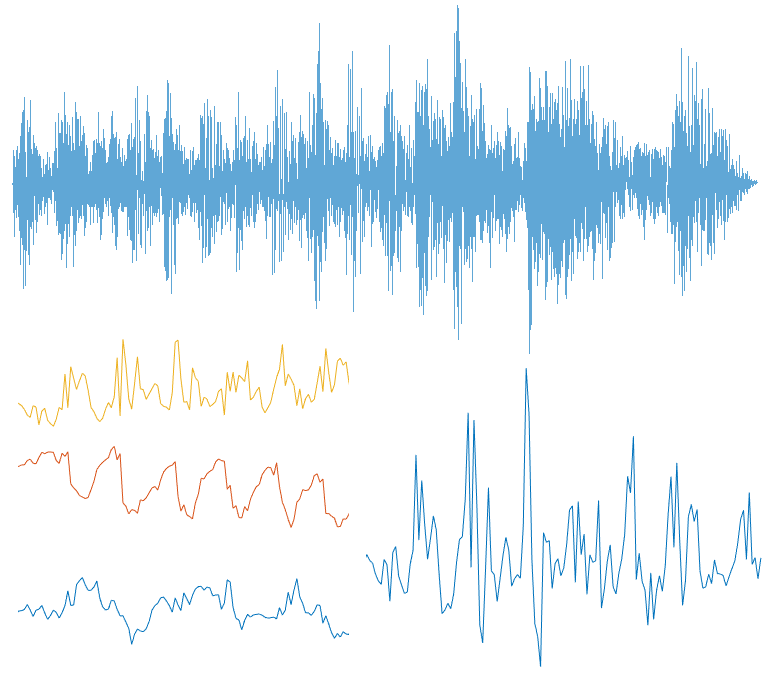
\includegraphics[width=0.9\linewidth]{app_example.png}
			\end{figure}
		\end{minipage}
		
\end{frame}
%--------------------------------------------------------------------------------
\begin{frame}{Related work}
	\begin{enumerate}
		\item Wang W. et al. Human activity recognition using smart phone embedded sensors: A Linear Dynamical Systems method. \emph{Neural Networks (IJCNN), 2014 International Joint Conference on (pp. 1185-1190)}. IEEE.
		\vspace{\baselineskip}
		\item Kwapisz J.~R., Weiss G.~M., Moore S.~A. Activity recognition using cell phone accelerometers. \emph{ACM SigKDD Explorations Newsletter}, 12(2), 74-82, 2011
		\vspace{\baselineskip}
		\item Kuznetsov M. P., Ivkin N. P. Time series classification algorithm using combined feature description. \emph{Journal of Machine Learning and Data Analysis}, 2015.
	\end{enumerate}
	
\end{frame}
%--------------------------------------------------------------------------------
%\section{Problem Statement}
\begin{frame}{Problem Statement}
	\textbf{Let:} $s \in \mathcal{S}$~--- complex structured object;\\
	\hspace{24pt}$y \in Y$ - class label;
	\vfill
	\begin{block}{Task}
	Suppose to be given the set of labeled data $\mathfrak{D} = \{(s_i, y_i)\}_{i=1}^m$. \\Our goal is to determine function $f^*$ such that \vspace{-0.2cm}$$f^* = \arg \min_f L\left(f, \mathfrak{D}\right),\vspace{-0.3cm}$$ where $L(\cdot, \cdot)$ is an error function and $f: \mathcal{S} \rightarrow Y$.
	\end{block}
	\vfill
	\begin{block}{Approach}
		Suppose $f = g \circ h$, where
		\begin{enumerate}
			\item $h(s): \mathcal{S} \rightarrow H \subset \mathbb{R}^n$ is map from $\mathcal{S}$ into feature space $H$;
			\item $g(\bm{h}, \bm\theta): H \rightarrow Y$ is parametric map (classification model).
		\end{enumerate}
	\end{block}
\end{frame}
%--------------------------------------------------------------------------------
\begin{frame}{Optimal parameters}
	
	\begin{minipage}[t]{0.15\columnwidth}
		\vspace{-0.6cm}
		\begin{block}{}
			\centering
			\vspace{0.5cm}
			$\,\,h(s)$
			\vspace{0.5cm}
		\end{block}
	\end{minipage}	
	\hfill
	\begin{minipage}[t]{0.8\columnwidth}
			Choice of feature map $h(s)$ by 
			\begin{itemize}
				\item prior (expert) knowledge;
				\item minimizing error functional.
			\end{itemize}
	\end{minipage}
\vfill
	\begin{minipage}[t]{0.15\columnwidth}
		\vspace{-0.6cm}
		\begin{block}{}
			\centering
			\vspace{1.3cm}
			$\,\,g(\bm{h}, \bm\theta)$
			\vspace{1.3cm}
		\end{block}
	\end{minipage}	
	\hfill
	\begin{minipage}[t]{0.8\columnwidth}
			Classification for $\{(\bm{h}_i , y_i)\}_{i=1}^m$, $\bm{h}_i = h(s_i)$:
			\[
				\bm{\theta}^* = \arg \min_{\bm\theta} L(g, \bm\theta, \mathfrak{D}).
			\]
		E.g.: $g(\mathbf{h}, \bm\theta)$ - classification model;
		
		\hspace{0.9cm}$\bm\theta$ - model parameters;
				
		\hspace{0.9cm}$L (g, \bm\theta, \mathfrak{D})$ - classification error function.
	\end{minipage}	

	

\end{frame}
%--------------------------------------------------------------------------------
\begin{frame}{Time series example}
	\begin{figure}[h]
		\centering
		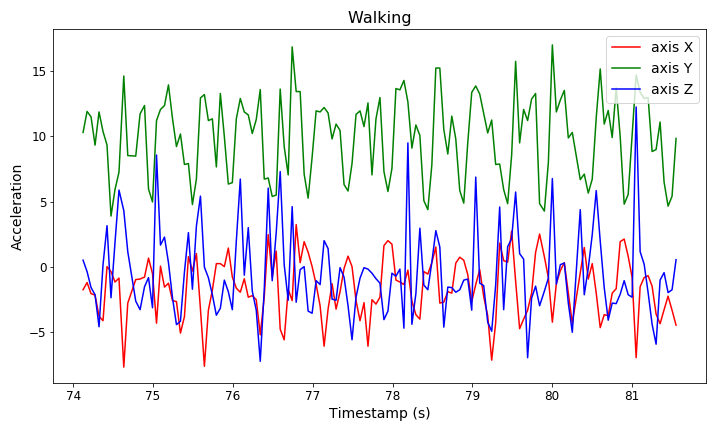
\includegraphics[width=1\linewidth]{ts_example.png}
		\label{ts_example}
	\end{figure}
\end{frame}
%--------------------------------------------------------------------------------
%\section{Feature extraction}
\begin{frame}{Expert functions}
	\textbf{Prior knowledge} about the objects allows to choose the features.
	\vfill
	\begin{block}{Feature description}
		$\bm{h}_i = h\left(s_i\right)\in \mathbb{R}^{40}$~--- different statistics:
		
		\hspace{0.5cm}\fbox{{\scriptsize 3}}$\:\,$ average accelerations;\\
		\hspace{0.5cm}\fbox{{\scriptsize 3}}$\:\,$ standard deviations;\\
		\hspace{0.5cm}\fbox{{\scriptsize 3}}$\:\,$ mean absolute deviations;\\
		\hspace{0.5cm}\fbox{{\scriptsize 1}}$\:\,$ average acceleration;\\
		\hspace{0.5cm}\fbox{{\scriptsize 30}} values of histogram with 10 equal parts.
	\end{block}

\end{frame}
%--------------------------------------------------------------------------------
\begin{frame}{Autoregressive model}
	\textbf{Data generation hypothesis}
	
		Let's assume that time series $s = (x_1, \dots, x_\T)$ is generated by the following autoregressive model:
		\[
			\widehat{x}_t = w_0 + \sum_{j=1}^n w_j x_{t-j}.
		\]
	\vfill
	\begin{block}{Feature description}
		\[
			h(s) = \mathbf{w}^* = \arg \min_{\mathbf{w} \in \mathbb{R}^{n+1}} \sum_{j=n+1}^{T} \left\| x_j - \hat{x}_j \right\|^2.
		\]
	\end{block}
\end{frame}
%--------------------------------------------------------------------------------
\begin{frame}{Singular Spectrum Analysis (SSA)}
	
	Let's consider a \textbf{trajectory matrix} for time series $s = (x_1, \dots, x_\T)$:
	\[
		\mathbf{X} = 
		\begin{pmatrix}
			x_1 & x_2 & \dots & x_n \\
			x_2 & x_3 & \dots & x_{n+1} \\
			\vdots & \vdots & \ddots & \vdots\\
			x_{\T-n+1} & x_{\T-n+2} & \dots & x_{\T}
		\end{pmatrix}
	\]
	\vfill
	\begin{block}{Feature description}
		\[
			h(s) = \left(\lambda_1, \dots ,\lambda_n\right),
		\]
		where $\{\lambda_i\}_{i=1}^n$ are eigenvalues of the matrix $\mathbf{X}^{\T} \mathbf{X}$, obtained by Singular Value Decomposition:
		$
			\mathbf{X}^{\T} \mathbf{X} = \mathbf{V} \cdot \text{diag} (\lambda_1, \dots, \lambda_n) \cdot \mathbf{V}^{\T}.
		$
	\end{block}

\end{frame}
%--------------------------------------------------------------------------------
\begin{frame}{(?!) Splines}
	
\end{frame}
%--------------------------------------------------------------------------------
\begin{frame}{Data}
\noindent
\begin{minipage}[t]{0.45\linewidth}
	\textbf{WISDM}$^1$
	\begin{table}[]
		\scriptsize
		\label{my-label}
		\begin{tabular}{l|rr}
			\hline
			\textbf{Activity}   & \multicolumn{2}{l}{\textbf{\# objects}} \\
			\hline
			Standing   & 229 & 5.3\% \\
			Walking    & 1917 & 44.4\%\\
			Upstairs   & 466 &10.8\%\\
			Sitting    & 277  &6.4\%\\
			Jogging    & 1075 &24.9\%\\
			Downstairs & 357 &8.3\%\\
			\hline
			Total & \multicolumn{2}{l}{4321}  \\
			\hline
		\end{tabular}
	\end{table}

	\vspace{1cm}
	\medskip\hrule\medskip
	{\scriptsize $^1$http://www.cis.fordham.edu/wisdm/ \\
		$^2$http://sipi.usc.edu/HAD/}
	
\end{minipage}
\hspace{-0.65cm}
\begin{minipage}[t]{0.02\columnwidth}
	\vspace{0.78cm}
	\begin{figure}[h]
		\centering
		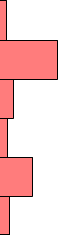
\includegraphics[width=2.3\linewidth]{hist1.png}
	\end{figure}
\end{minipage}
\hfill
\begin{minipage}[t]{0.47\linewidth}
	\textbf{USC-HAD}$^2$
	\begin{table}[]
		\scriptsize
		\label{my-label}
		\begin{tabular}{l|rr}
			\hline
			\textbf{Activity} & \multicolumn{2}{l}{\textbf{\# objects}} \\ \hline
			Walking-downstairs & 951 & 7\%  \\
			Walking-upstairs        & 1018&7.4\%  \\
			Walking-forward    & 1874&13.8\% \\
			Walking-right        & 1305&9.6\%  \\
			Walking-left        & 1280&9.4\%  \\
			Elevator-up        & 764&5.6\% \\
			Elevator-down        & 763&5.6\%  \\
			Standing           & 1167&8.6\%  \\
			Sitting            & 1294&9.5\%  \\
			Sleeping           & 1860&13.7\% \\
			Jumping        & 495&3.6\%  \\
			Running            & 849&6.2\%  \\ \hline 
			Total              & \multicolumn{2}{l}{13620}\\ 
			\hline
		\end{tabular}
	\end{table}
\end{minipage}
\hspace{-0.24cm}
\begin{minipage}[t]{0.02\columnwidth}
	\vspace{0.78cm}
	\begin{figure}[h]
		\centering
		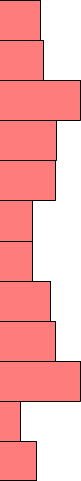
\includegraphics[width=3.135\linewidth]{hist2.png}
	\end{figure}
\end{minipage}

\end{frame}
%--------------------------------------------------------------------------------
\begin{frame}{Experiment}
		\begin{align*}
			\text{\textbf{Datasets: }} &\text{WISDM, USC-HAD;}\\
		\text{\textbf{Feature extraction methods: }} &\text{expert functions;}\\ &\text{autoregressive models;}\\ &\text{singular spectral analysis;}\\ &\text{splines;}\\
		\text{\textbf{Classification models:} } &\text{logistic regression;}\\ &\text{support vector machine;}\\ &\text{random forest;}\\
		\text{\textbf{Tuning parameters: }} &\text{cross-validation;}\\
		\text{\textbf{Quality measure: }} &\text{accuracy score.}
		\end{align*}

\end{frame}
%--------------------------------------------------------------------------------
\begin{frame}{Results}
	\begin{table}[]
		\centering
		\label{my-label}
		\begin{tabular}{|l|c|c|c|c|}
			\hline
			 & Expert & AutoReg & SSA & Splines\\
			\hline
			Log-Reg &    0.668    &    0.651     &   0.637  & 0.415  \\
			\hline
			SVM     &    0.797    &     0.655    &   0.822  & 0.740\\
			\hline
			RF      &    0.871    &     0.703    &  0.840 & 0.736 \\
			\hline
		\end{tabular}
	\end{table}

\end{frame}
%--------------------------------------------------------------------------------
\begin{frame}{Feature union}

\end{frame}
%--------------------------------------------------------------------------------
\begin{frame}{Conclusion}
	\begin{block}{Done}
		\begin{itemize}
			\item different approaches to classification of complex-structured objects were studied
			\item the results of experiments on human activities datasets outperform many previous methods
			\item 
		\end{itemize}
	\end{block}
	\begin{block}{Future work}
		\begin{itemize}
			\item new approaches to feature extraction (e.g. modified splines)
			\item implementing of structured learning methods
		\end{itemize}
	
	\end{block}
\end{frame}


\end{document} 